%=======================================================================
%  SERIES DE FOURIER - METODO TRIGONOMETRICO Y EXPONENCIAL COMPLEJO
%  Curso : Senales y Sistemas  (2026-2)
%  UCSP  - Facultad de Ingenieria - Ing. Electronica y de Telecomunicaciones
%  Docente     : (por confirmar)
%  Jefe de practica / autor : Ing. Jeanpier Ancori Sanchez
%
%  Material de CLASE (Contenidos/Series_de_Fourier/), no guia de laboratorio:
%  por eso la cabecera no lleva Nota, Grupo ni Alumno(s), y no hay puntajes ni
%  lineas de respuesta salvo en los ejercicios propuestos del final. El
%  documento es la version impresa del notebook
%  01_Serie_trigonometrica_y_compleja.ipynb: mismo ejercicio, mismos pasos,
%  mismos numeros. Si uno cambia, hay que cambiar el otro.
%
%  Version 1 - Un unico ejercicio resuelto por los dos metodos.
%
%  EL EJERCICIO. f(t) = t en (-pi, pi), T = 2 pi. Se elige porque es la
%  senal mas corta que obliga a las dos ideas dificiles a la vez: la paridad
%  (a_n = 0 sin integrar) y la integracion por partes (b_n y C_n). Con
%  T = 2 pi ademas w0 = 1 y los armonicos son sen(nt) a secas; el texto avisa
%  de que eso es una coincidencia del ejercicio y no la regla.
%
%  POR QUE UN SOLO EJERCICIO. Resolver el mismo problema por los dos caminos
%  es lo que permite DEMOSTRAR la equivalencia en vez de afirmarla: el alumno
%  ve que C_n sale igual por integracion directa (seccion V) que por la
%  formula C_n = (a_n - j b_n)/2 (seccion VI). Dos ejercicios distintos
%  habrian dejado la coincidencia sin comprobar.
%
%  NIVEL. Alumnos de primeros semestres: no se supone que conocen Euler. La
%  identidad se deduce (sumando y restando) antes de usarla, y la propiedad
%  de las integrales de funciones impares se demuestra con el cambio t -> -t
%  en lugar de citarla. Las identidades que suelen olvidarse van en el
%  apendice.
%
%  ERRATA DEL ENCARGO ORIGINAL. El texto de partida escribia los limites de
%  a_n y b_n como "-T/2 a T"; es un descuido, el periodo es de -T/2 a T/2 y
%  asi esta aqui. No se corrigio en silencio en ninguna otra parte: el resto
%  de formulas del encargo se comprobaron una a una (ver abajo).
%
%  VERIFICACION. Todos los coeficientes se comprobaron aparte, antes de
%  escribir el texto, con integrales numericas de 200 000 puntos: b_n =
%  2, -1, 2/3, -1/2, 2/5; C_n = j(-1)^n/n; C_{-n} = C_n^*; la serie trigono-
%  metrica y la compleja coinciden a 1e-15; Parseval da pi^2/3 por los dos
%  lados. El sobrepico de Gibbs sube a ~8,85 % del salto con N = 500, cerca
%  del ~9 % teorico; con N = 5 todavia no se ha formado (0,38 %), y por eso
%  el texto dice "alrededor del 9 %" sin dar un valor para N = 5.
%
%  FIGURAS. Las genera Codigo/generar_figuras.py en PDF vectorial y con
%  Trebuchet MS. En el salto de la senal se dibujan los dos extremos huecos
%  (f no esta definida en +-pi) y el valor al que converge la serie, 0, en
%  rojo: es la imagen de "promedio de los limites laterales".
%
%  LISTADO DE CODIGO. Con fancyvrb (Verbatim), no con listings: listings con
%  XeLaTeX y UTF-8 exige configuracion aparte para tildes y enes, y aqui los
%  comentarios del codigo estan en castellano. Hay que cuidar que las lineas
%  no pasen de ~100 caracteres en cuerpo \footnotesize.
%
%  Version 2 - Apendice de identidades y Parseval.
%  Lo pide el autor: "agrega alguna identidad que quiza no he agregado".
%  Entran: potencias de j, De Moivre, producto a suma, forma amplitud-fase,
%  ortogonalidad de los armonicos (que es lo que justifica las formulas de los
%  coeficientes) y Parseval, que ademas sirve de comprobacion independiente
%  de los C_n.
%
%  Version 3 - Ejercicios mas sencillos y un ejercicio completo.
%  Lo pide el autor: los propuestos eran demasiado dificiles (error cuadratico
%  medio, cambiar el periodo en el codigo) y faltaba uno donde el alumno haga
%  TODO el recorrido por su cuenta. Ahora hay dos partes. La A son cinco
%  ejercicios de una sola idea (frecuencias, paridad, Euler en ambos sentidos,
%  valor en un salto). La B repite el recorrido completo con la onda cuadrada,
%  guiado en 8 pasos.
%
%  POR QUE LA ONDA CUADRADA. Es la mas facil con la que se llega a las dos
%  series: es impar (a_n = 0 sin integrar) y b_n sale de integrar sen(nt), sin
%  integracion por partes. Se descartaron |t| (pide partes y tiene a_n distinto
%  de cero, es otro nivel) y el pulso en (0, pi) (no es ni par ni impar, hay que
%  calcular a_n y b_n). Ademas tiene lo que ensena la diente de sierra mas un
%  detalle nuevo: los armonicos pares valen cero, y el alumno debe separar n par
%  de n impar. Para que se vea como se pide el paso 3, la primera fila de la
%  tabla viene resuelta (n = 1) y el codigo trae la pista de np.where.
%
%  RESPUESTAS. Van en pagina aparte para que no se lean sin querer. Todas se
%  comprobaron numericamente antes de escribirlas: b_n = 4/(n pi) en impares,
%  C_n = -2j/(n pi), la serie vale 1 en t = pi/2 (serie de Leibniz), el
%  sobrepico de Gibbs es 8,95 % del salto a N = 200 (pico 1,179) y Parseval da
%  1 por los dos lados.
%=======================================================================

\documentclass[11pt,a4paper]{article}

%------------------------------------------------------------- idioma
% Compilar con XeLaTeX (no con pdflatex): Trebuchet MS es una fuente TrueType
% del sistema y solo fontspec, bajo XeLaTeX o LuaLaTeX, sabe cargarla.
% inputenc y fontenc se omiten a proposito: XeLaTeX trabaja en UTF-8 de forma
% nativa y esos paquetes dan error con este motor.
\usepackage{fontspec}
\setmainfont{Trebuchet MS}[
  Path            = C:/Windows/Fonts/,
  Extension       = .ttf,
  UprightFont     = trebuc,
  BoldFont        = trebucbd,
  ItalicFont      = trebucit,
  BoldItalicFont  = trebucbi,
  Ligatures       = TeX
]
\setmonofont{Consolas}[
  Path            = C:/Windows/Fonts/,
  Extension       = .ttf,
  UprightFont     = consola,
  BoldFont        = consolab,
  ItalicFont      = consolai,
  BoldItalicFont  = consolaz,
  Scale           = 0.92
]
\usepackage[spanish,es-nodecimaldot]{babel}
\usepackage{microtype}

%----------------------------------------------------------- geometria
\usepackage[left=2.4cm,right=2.4cm,top=3.1cm,bottom=2.6cm,headheight=30pt,
            footskip=1.2cm]{geometry}

%------------------------------------------------------------ graficos
\usepackage{graphicx}
\usepackage{float}
\usepackage{placeins}
\usepackage[font=small,labelfont=bf,labelsep=period]{caption}
\graphicspath{{imagenes/}}

%-------------------------------------------------------------- tablas
\usepackage{array}
\usepackage{tabularx}
\usepackage{booktabs}

%----------------------------------------------------- matematicas / SI
\usepackage{amsmath,amssymb}
\usepackage{siunitx}
\sisetup{
  output-decimal-marker = {,},
  per-mode              = symbol,
  range-phrase          = { a },
  range-units           = single,
  mode                  = match,
  detect-weight         = true,
  detect-family         = true
}
% En castellano el seno es "sen", no "sin".
\DeclareMathOperator{\sen}{sen}
\DeclareMathOperator{\Real}{Re}
\DeclareMathOperator{\Imag}{Im}

%--------------------------------------------------------------- listas
\usepackage{enumitem}
\setlist[itemize]{itemsep=3pt,topsep=4pt,parsep=0pt}
\setlist[enumerate]{itemsep=8pt,topsep=4pt,parsep=0pt}

%--------------------------------------------------------------- cajas
\usepackage[most]{tcolorbox}
\usepackage{pgffor}

\newtcolorbox{notatec}[1]{enhanced,breakable,
  colback=blue!3!white, colframe=blue!55!black,
  fonttitle=\bfseries\small, title={Nota técnica --- #1},
  boxrule=0.6pt, arc=2pt, left=6pt,right=6pt,top=4pt,bottom=4pt}

\newtcolorbox{seguridad}[1]{enhanced,breakable,
  colback=red!3!white, colframe=red!60!black,
  fonttitle=\bfseries\small, title={Seguridad --- #1},
  boxrule=0.6pt, arc=2pt, left=6pt,right=6pt,top=4pt,bottom=4pt}

\newtcolorbox{ejemplo}[1]{enhanced,breakable,
  colback=green!3!white, colframe=green!45!black,
  fonttitle=\bfseries\small, title={Ejemplo resuelto --- #1},
  boxrule=0.6pt, arc=2pt, left=6pt,right=6pt,top=4pt,bottom=4pt}

%---------------------------------------------------------------- codigo
\usepackage{fancyvrb}
\fvset{fontsize=\footnotesize,frame=single,framesep=3mm,rulecolor=\color{black!35},
       baselinestretch=1.0,numbers=left,numbersep=5pt}
\newcommand{\py}[1]{\texttt{#1}}

%------------------------------------------------------------ comandos
% Lineas punteadas para respuestas del alumno: \lineasresp{n}
\newcommand{\lineasresp}[1]{%
  \par\vspace{6pt}%
  \foreach \i in {1,...,#1}{\noindent\rule{\linewidth}{0.4pt}\par\vspace{11pt}}%
}

%----------------------------------------------------- compaginacion
\usepackage{needspace}
\usepackage{etoolbox}
\pretocmd{\section}{\needspace{5\baselineskip}}{}{}
\pretocmd{\subsection}{\needspace{4\baselineskip}}{}{}
\widowpenalty=10000
\clubpenalty=10000

%------------------------------------------------------------ espaciado
\setlength{\intextsep}{9pt}
\setlength{\abovecaptionskip}{6pt}
\AtBeginDocument{%
  \setlength{\abovedisplayskip}{7pt}%
  \setlength{\belowdisplayskip}{7pt}%
  \setlength{\abovedisplayshortskip}{4pt}%
  \setlength{\belowdisplayshortskip}{4pt}%
}

%---------------------------------------------------- encabezado / pie
\usepackage{fancyhdr}
\pagestyle{fancy}
\fancyhf{}
\fancyhead[L]{\footnotesize UCSP --- Facultad de Ingeniería\\
              Ing. Electrónica y de Telecomunicaciones}
\fancyhead[R]{\footnotesize 2026-2 Señales y Sistemas\\
              Jeanpier Ancori Sánchez}
\fancyfoot[L]{\footnotesize Material de clase --- Series de Fourier}
\fancyfoot[R]{\footnotesize Página \thepage\ de \pageref{LastPage}}
\renewcommand{\headrulewidth}{0.4pt}
\renewcommand{\footrulewidth}{0.4pt}
\usepackage{lastpage}

%------------------------------------------------------- numeracion
\renewcommand{\thesection}{\Roman{section}}
\renewcommand{\thesubsection}{\arabic{section}.\arabic{subsection}}
\renewcommand{\thesubsubsection}{\thesubsection.\arabic{subsubsection}}
\setcounter{secnumdepth}{3}

%-------------------------------------------------------- hiperenlaces
\usepackage[hidelinks,pdfusetitle]{hyperref}
\usepackage{xurl}
\hypersetup{
  pdftitle={Series de Fourier - Metodo trigonometrico y exponencial complejo},
  pdfsubject={Senales y Sistemas - Material de clase},
  pdfauthor={Jeanpier Ancori Sanchez},
  pdfkeywords={senales y sistemas, serie de Fourier, exponencial compleja,
               identidad de Euler, frecuencias negativas, fenomeno de Gibbs}
}

% babel-spanish rotula las tablas como "Cuadro"; los originales dicen "Tabla".
\addto\captionsspanish{\renewcommand{\tablename}{Tabla}}

\begin{document}

%=======================================================================
%  CABECERA
%=======================================================================
\begingroup
\renewcommand{\tabularxcolumn}[1]{m{#1}}
\renewcommand{\arraystretch}{2.0}
\setlength{\tabcolsep}{12pt}
\noindent
\begin{tabularx}{\textwidth}{|>{\centering\arraybackslash}m{2.2cm}|>{\centering\arraybackslash}X|}
\hline
\rule{0pt}{2.1cm}{\fontsize{58}{58}\selectfont\bfseries $\sum$}
    & \begin{minipage}[c]{\linewidth}\centering
          {\large\bfseries Material de clase}\\[7pt]
          {\Large\bfseries Series de Fourier:\\
           método trigonométrico y\\ exponencial complejo}
      \end{minipage}\\
\hline
\multicolumn{2}{|l|}{\rule{0pt}{1.1cm}\large\textbf{Curso:}~Señales y Sistemas \hfill
    \textbf{Periodo:}~2026-2\hspace{2mm}}\\
\hline
\end{tabularx}
\endgroup

\vspace{0.8cm}

%=======================================================================
\section{Objetivos}
%=======================================================================
Al terminar este documento el alumno será capaz de:

\begin{itemize}
    \item Explicar qué es una serie de Fourier y distinguir período, frecuencia
          fundamental, frecuencia angular, armónicos y componente continua.
    \item Calcular los coeficientes $a_0$, $a_n$ y $b_n$ de la serie
          trigonométrica de una señal periódica, usando paridad e integración
          por partes.
    \item Calcular los coeficientes $C_n$ de la serie exponencial compleja.
    \item \textbf{Demostrar} la relación entre ambos conjuntos de coeficientes a
          partir de las identidades de Euler, y no solo afirmarla.
    \item Interpretar las frecuencias positivas y negativas y la simetría
          conjugada $C_{-n}=C_n^{*}$.
    \item Reconstruir la señal con un número finito de armónicos y reconocer el
          fenómeno de Gibbs.
\end{itemize}

Se resuelve \textbf{un único ejercicio} por los dos métodos, para que se vea que
son dos formas de escribir lo mismo.

\begin{notatec}{requisitos}
Se supone conocida la exponencial compleja de la Semana 4 y la integración por
partes. \emph{No} se supone que el alumno conozca las identidades de Euler: se
deducen en la sección~\ref{sec:equivalencia}.
\end{notatec}

\FloatBarrier
%=======================================================================
\section{Marco teórico}
%=======================================================================

\subsection{Qué es una serie de Fourier}
Una \textbf{serie de Fourier} representa una señal periódica como una \textbf{suma
de senos y cosenos} (o, de forma equivalente, de exponenciales complejas) cuyas
frecuencias son \textbf{múltiplos enteros de una frecuencia básica}. La idea
central: cualquier señal periódica ``razonable'' se puede construir sumando
ondas senoidales simples, cada una con la amplitud y la fase adecuadas.

\subsection{Definiciones}
\begin{table}[H]
\centering
\caption{Vocabulario de la serie de Fourier.}
\renewcommand{\arraystretch}{1.5}
\begin{tabularx}{\textwidth}{>{\raggedright\arraybackslash}p{3.7cm}cXl}
\toprule
\textbf{Concepto} & \textbf{Símbolo} & \textbf{Significado} & \textbf{En este ejercicio}\\
\midrule
Período & $T$ & Menor tiempo tras el cual la señal se repite: $f(t+T)=f(t)$ &
  $T=2\pi$ s\\
Frecuencia fundamental & $f_0=1/T$ & Períodos por segundo, en Hz &
  $f_0=\dfrac{1}{2\pi}\approx\qty{0.159}{\hertz}$\\
Frecuencia angular fundamental & $\omega_0=2\pi f_0$ & La misma frecuencia en rad/s &
  $\omega_0=\qty{1}{\radian\per\second}$\\
Armónico $n$ & $n\omega_0$ & Onda de frecuencia $n$ veces la fundamental
  ($n=1,2,3,\dots$); el armónico 1 es la fundamental & $n\cdot\qty{1}{\radian\per\second}$\\
Componente continua (DC) & $a_0/2$ & Valor promedio de la señal; componente de
  frecuencia cero & se calcula en~\ref{sec:a0}\\
\bottomrule
\end{tabularx}
\end{table}

\subsection{La frecuencia angular fundamental}
La relación que enlaza período y frecuencia angular es
\begin{equation*}
  \boxed{\omega_0=\frac{2\pi}{T}}
\end{equation*}
Para este ejercicio, con $T=2\pi$:
\begin{equation*}
  \omega_0=\frac{2\pi}{2\pi}=\qty{1}{\radian\per\second}
\end{equation*}
Esto simplifica todo: los armónicos son $\cos(nt)$ y $\sen(nt)$ en lugar de
$\cos(n\omega_0t)$ y $\sen(n\omega_0t)$. \textbf{Cuidado:} es una coincidencia de
este ejercicio ($T=2\pi$); en general $\omega_0\neq 1$.

\FloatBarrier
%=======================================================================
\section{Enunciado del ejercicio}
%=======================================================================
Considera la señal periódica definida en un período por
\begin{equation*}
  \boxed{f(t)=t,\qquad -\pi<t<\pi}
  \qquad\text{con extensión periódica}\qquad
  \boxed{T=2\pi}
\end{equation*}
es decir, $f(t+2\pi)=f(t)$ fuera de $(-\pi,\pi)$. Su gráfica es una \textbf{onda
diente de sierra} (figura~\ref{fig:senal}).

\begin{figure}[H]
\centering
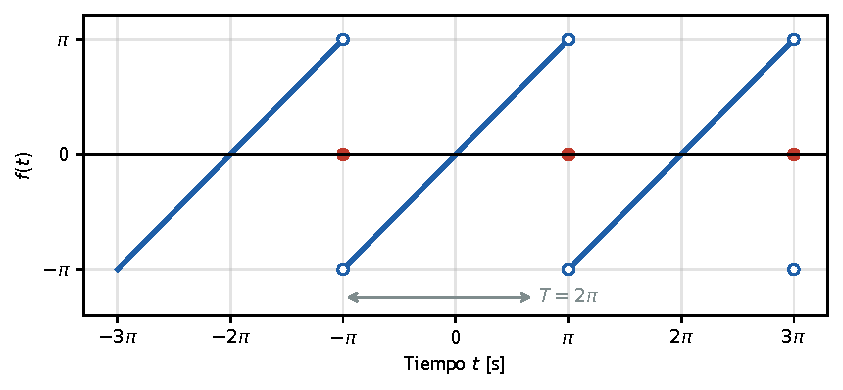
\includegraphics[width=0.92\linewidth]{senal_original.pdf}
\caption{Señal $f(t)=t$ en $(-\pi,\pi)$ repetida con $T=2\pi$. En cada salto
$f$ no está definida en $\pm\pi$ (extremos huecos); el punto rojo es el valor
al que converge la serie, el promedio de los límites laterales.}
\label{fig:senal}
\end{figure}

\textbf{Se pide determinar:}
\begin{enumerate}[label=\arabic*.]
    \item La serie de Fourier \textbf{trigonométrica}.
    \item La serie de Fourier \textbf{exponencial compleja}.
    \item Los coeficientes de ambas representaciones.
    \item La equivalencia matemática entre los resultados.
    \item La aproximación de la señal con los primeros armónicos.
\end{enumerate}

\FloatBarrier
%=======================================================================
\section{Resolución por el método trigonométrico}
%=======================================================================

\subsection{La forma de la serie y las fórmulas de los coeficientes}
\begin{equation*}
  \boxed{f(t)=\frac{a_0}{2}+\sum_{n=1}^{\infty}\Big[a_n\cos(n\omega_0t)+b_n\sen(n\omega_0t)\Big]}
\end{equation*}
\begin{itemize}
    \item $a_0/2$: componente continua (valor promedio).
    \item $a_n$: amplitud del \textbf{coseno} del armónico $n$.
    \item $b_n$: amplitud del \textbf{seno} del armónico $n$.
\end{itemize}
Los coeficientes se obtienen proyectando la señal sobre cada armónico, integrando
en \textbf{un período completo} (aquí de $-T/2$ a $T/2$):
\begin{align*}
  \boxed{a_0=\frac{2}{T}\int_{-T/2}^{T/2}f(t)\,dt}\qquad
  \boxed{a_n=\frac{2}{T}\int_{-T/2}^{T/2}f(t)\cos(n\omega_0t)\,dt}\qquad
  \boxed{b_n=\frac{2}{T}\int_{-T/2}^{T/2}f(t)\sen(n\omega_0t)\,dt}
\end{align*}
Con $T=2\pi$ el factor $2/T$ vale $1/\pi$ y los límites son $-\pi$ y $\pi$.

\subsection{Cálculo de \texorpdfstring{$a_0$}{a0}}\label{sec:a0}
\begin{align*}
  a_0&=\frac{1}{\pi}\int_{-\pi}^{\pi}t\,dt
     =\frac{1}{\pi}\left[\frac{t^{2}}{2}\right]_{-\pi}^{\pi}
     =\frac{1}{\pi}\left(\frac{\pi^{2}}{2}-\frac{(-\pi)^{2}}{2}\right)
     =\frac{1}{\pi}\left(\frac{\pi^{2}}{2}-\frac{\pi^{2}}{2}\right)\\[4pt]
  &\boxed{a_0=0}
\end{align*}
\textbf{Significado físico:} $a_0/2$ es el \textbf{valor promedio} de la señal en un
período. La rampa toma valores negativos y positivos de forma simétrica: el área bajo
el eje cancela exactamente la de arriba y el promedio es cero. La señal \textbf{no
tiene componente continua}.

\subsection{Cálculo de \texorpdfstring{$a_n$}{an}: uso de la paridad}
Una función $g$ es \textbf{par} si $g(-t)=g(t)$ e \textbf{impar} si $g(-t)=-g(t)$. Para
el producto de dos funciones valen las mismas reglas que para los signos:

\begin{table}[H]
\centering
\caption{Paridad de un producto.}
\begin{tabular}{lc}
\toprule
\textbf{Producto} & \textbf{Resultado}\\
\midrule
par $\times$ par & par\\
impar $\times$ impar & par\\
par $\times$ impar & \textbf{impar}\\
\bottomrule
\end{tabular}
\end{table}

En $a_n$ el integrando es $t\cos(nt)$: $t$ es \textbf{impar}, $\cos(nt)$ es \textbf{par};
por tanto $g(t)=t\cos(nt)$ es \textbf{impar}.

\textbf{Por qué la integral de una función impar sobre un intervalo simétrico es cero.}
Se parte la integral en dos mitades y en la primera se cambia $t\to -t$:
\begin{equation*}
  \int_{-\pi}^{\pi}g(t)\,dt=\int_{-\pi}^{0}g(t)\,dt+\int_{0}^{\pi}g(t)\,dt
\end{equation*}
Con $u=-t$ y $dt=-du$ (los límites $t=-\pi\to u=\pi$ y $t=0\to u=0$):
\begin{equation*}
  \int_{-\pi}^{0}g(t)\,dt=-\int_{\pi}^{0}g(-u)\,du=\int_{0}^{\pi}g(-u)\,du=-\int_{0}^{\pi}g(u)\,du
\end{equation*}
(la última igualdad usa que $g$ es impar). Al sumar, las dos mitades se cancelan:
\begin{equation*}
  \int_{-\pi}^{\pi}t\cos(nt)\,dt=0\quad\Longrightarrow\quad
  \boxed{a_n=\frac{1}{\pi}\int_{-\pi}^{\pi}t\cos(nt)\,dt=0}
\end{equation*}
Vale para todo $n\ge 1$: \textbf{ningún coseno aparece en la serie}. Es lo esperable:
$f(t)=t$ es impar y los cosenos (pares) no pueden aportar a una función impar.

\subsection{Cálculo de \texorpdfstring{$b_n$}{bn}}
El integrando es $t\sen(nt)$: $t$ es impar y $\sen(nt)$ es impar, así que el producto
es \textbf{par}. En una función par las dos mitades de la integral son iguales y se suman:
\begin{equation*}
  \int_{-\pi}^{\pi}t\sen(nt)\,dt=2\int_{0}^{\pi}t\sen(nt)\,dt
  \quad\Longrightarrow\quad
  \boxed{b_n=\frac{2}{\pi}\int_{0}^{\pi}t\sen(nt)\,dt}
\end{equation*}

\textbf{Integración por partes.} La regla es $\displaystyle\int u\,dv=uv-\int v\,du$.
Se elige $u$ como la parte que se simplifica al derivar ($t$) y $dv$ como la que se
sabe integrar ($\sen(nt)\,dt$):
\begin{align*}
  u&=t &\Rightarrow\quad du&=dt\\
  dv&=\sen(nt)\,dt &\Rightarrow\quad v&=-\frac{\cos(nt)}{n}
\end{align*}
Se sustituye:
\begin{align*}
  \int t\sen(nt)\,dt
  &=t\left(-\frac{\cos(nt)}{n}\right)-\int\left(-\frac{\cos(nt)}{n}\right)dt\\
  &=-\frac{t\cos(nt)}{n}+\frac{1}{n}\int\cos(nt)\,dt
   =-\frac{t\cos(nt)}{n}+\frac{\sen(nt)}{n^{2}}
\end{align*}
Entonces
\begin{equation*}
  b_n=\frac{2}{\pi}\left[-\frac{t\cos(nt)}{n}+\frac{\sen(nt)}{n^{2}}\right]_{0}^{\pi}
\end{equation*}
Se evalúa con $\cos(n\pi)=(-1)^{n}$ y $\sen(n\pi)=0$ ($n$ entero):
\begin{itemize}
    \item en $t=\pi$: $\;-\dfrac{\pi(-1)^{n}}{n}+\dfrac{0}{n^{2}}=-\dfrac{\pi(-1)^{n}}{n}$
    \item en $t=0$: $\;-\dfrac{0\cdot\cos 0}{n}+\dfrac{\sen 0}{n^{2}}=0$
\end{itemize}
\begin{equation*}
  b_n=\frac{2}{\pi}\left(-\frac{\pi(-1)^{n}}{n}-0\right)=-\frac{2(-1)^{n}}{n}
\end{equation*}
y como $-(-1)^{n}=(-1)^{n+1}$:
\begin{equation*}
  \boxed{b_n=\frac{2(-1)^{n+1}}{n}}
\end{equation*}

\begin{ejemplo}{comprobación con valores}
Para $n=1$: $b_1=2(-1)^{2}/1=2$. Para $n=2$: $b_2=2(-1)^{3}/2=-1$. Para $n=3$:
$b_3=2(-1)^{4}/3=\tfrac{2}{3}$. Estos tres valores coinciden con la integral calculada
numéricamente (suma de Riemann con \num{200000} puntos): \num{2,000000},
\num{-1,000000} y \num{0,666667}.
\end{ejemplo}

\subsection{Resultado trigonométrico}
Con $a_0=0$, $a_n=0$, $b_n=\dfrac{2(-1)^{n+1}}{n}$ y $\omega_0=1$:
\begin{equation*}
  \boxed{f(t)=2\sum_{n=1}^{\infty}\frac{(-1)^{n+1}}{n}\sen(nt)}
\end{equation*}
Los primeros términos:
\begin{equation*}
  f(t)=2\sen t-\sen 2t+\frac{2}{3}\sen 3t-\frac{1}{2}\sen 4t+\frac{2}{5}\sen 5t-\cdots
\end{equation*}

\textbf{Cómo se construye y qué representa cada término.} El primero, $2\sen t$, es la
\textbf{fundamental}: una senoidal con el mismo período que la señal (da la forma
general de subida y bajada). Cada término siguiente es un \textbf{armónico} que oscila
más rápido y con amplitud menor ($|b_n|=2/n$ decrece como $1/n$); su función es
\emph{corregir} la forma: el signo alterno $(-1)^{n+1}$ hace que unos armónicos sumen y
otros resten, y entre todos ``enderezan'' la suma hasta parecerse a la rampa y a su caída
brusca (figura~\ref{fig:armonicos}).

\begin{figure}[H]
\centering
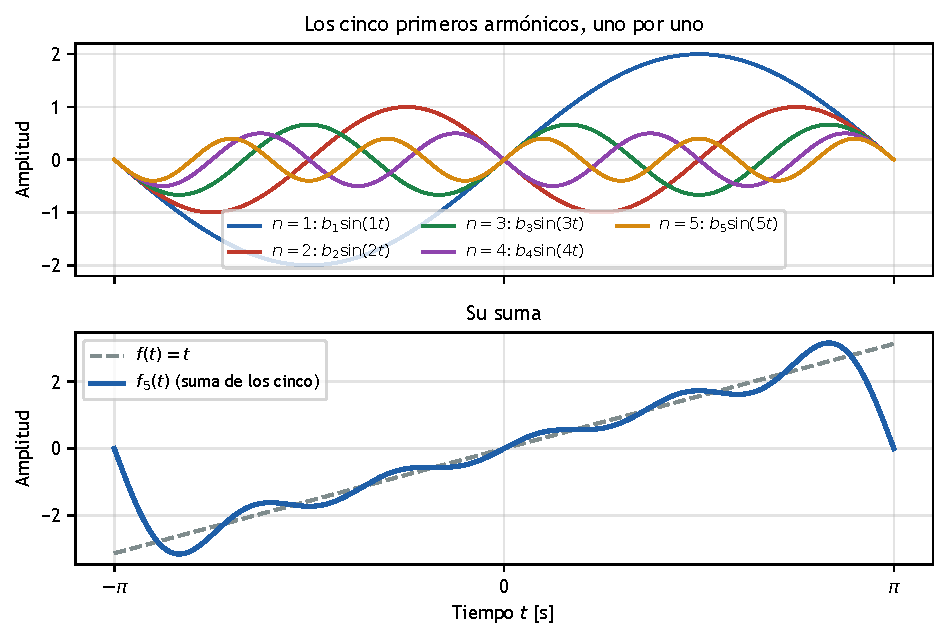
\includegraphics[width=0.95\linewidth]{armonicos.pdf}
\caption{Arriba, los cinco primeros términos de la serie por separado. Abajo, su suma
$f_5(t)$ frente a la señal original.}
\label{fig:armonicos}
\end{figure}

\FloatBarrier
%=======================================================================
\section{Resolución mediante exponenciales complejas}
%=======================================================================

\subsection{La forma compleja}
\begin{equation*}
  \boxed{f(t)=\sum_{n=-\infty}^{\infty}C_n\,e^{jn\omega_0t}}
\end{equation*}
Aquí $C_n$ es un número \textbf{complejo} (el coeficiente del armónico $n$) y
$e^{jn\omega_0t}$ es una exponencial compleja que gira con frecuencia $n\omega_0$. El
índice $n$ recorre \textbf{todos los enteros}, positivos y negativos; la
sección~\ref{sec:frecuencias} explica qué significa eso. Los coeficientes se calculan con
\begin{equation*}
  \boxed{C_n=\frac{1}{T}\int_{-T/2}^{T/2}f(t)\,e^{-jn\omega_0t}\,dt}
\end{equation*}
Con $T=2\pi$, $\omega_0=1$ y $f(t)=t$:
\begin{equation*}
  \boxed{C_n=\frac{1}{2\pi}\int_{-\pi}^{\pi}t\,e^{-jnt}\,dt}
\end{equation*}
\begin{notatec}{n distinto de cero}
La antiderivada que se obtiene a continuación tiene $n$ en el denominador, así que
\textbf{solo sirve para $n\neq 0$}. El caso $n=0$ ($C_0$) se calcula aparte, en la
sección~\ref{sec:c0}.
\end{notatec}

\subsection{Resolver la integral exponencial}
De nuevo, integración por partes:
\begin{align*}
  u&=t &\Rightarrow\quad du&=dt\\
  dv&=e^{-jnt}\,dt &\Rightarrow\quad v&=\frac{e^{-jnt}}{-jn}
\end{align*}
(La integral de $e^{at}$ es $e^{at}/a$; aquí $a=-jn$. El factor $j$ aparece porque la
constante del exponente es imaginaria.) Entonces
\begin{align*}
  \int te^{-jnt}\,dt
  &=t\cdot\frac{e^{-jnt}}{-jn}-\int\frac{e^{-jnt}}{-jn}\,dt
   =-\frac{te^{-jnt}}{jn}+\frac{1}{jn}\int e^{-jnt}\,dt\\
  &=-\frac{te^{-jnt}}{jn}+\frac{1}{jn}\cdot\frac{e^{-jnt}}{-jn}
   =-\frac{te^{-jnt}}{jn}+\frac{e^{-jnt}}{-j^{2}n^{2}}
\end{align*}
Como $j^{2}=-1$, el denominador $-j^{2}n^{2}$ vale $n^{2}$:
\begin{equation*}
  \boxed{\int te^{-jnt}\,dt=-\frac{te^{-jnt}}{jn}+\frac{e^{-jnt}}{n^{2}}}
\end{equation*}
\textbf{Origen de cada término:} el primero es $uv$, el producto $t\cdot v$; el segundo es
$-\int v\,du$, que al integrar otra vez una exponencial introduce un segundo factor
$1/(jn)$ y, junto con el que ya había, un $n^{2}$ en el denominador (el producto
$j\cdot j=-1$ elimina la unidad imaginaria).

\subsection{Evaluar los límites}
\begin{equation*}
  C_n=\frac{1}{2\pi}\left[-\frac{te^{-jnt}}{jn}+\frac{e^{-jnt}}{n^{2}}\right]_{-\pi}^{\pi}
\end{equation*}
Hacen falta $e^{-jn\pi}$ y $e^{jn\pi}$. Por Euler (sección~\ref{sec:euler}),
\begin{equation*}
  e^{\pm jn\pi}=\cos(n\pi)\pm j\sen(n\pi)=(-1)^{n}\pm j\cdot 0
  \quad\Longrightarrow\quad
  \boxed{e^{jn\pi}=e^{-jn\pi}=(-1)^{n}}
\end{equation*}
\textbf{Primer término}, $-\dfrac{te^{-jnt}}{jn}$:
\begin{itemize}
    \item en $t=\pi$: $\;-\dfrac{\pi(-1)^{n}}{jn}$
    \item en $t=-\pi$: $\;-\dfrac{(-\pi)(-1)^{n}}{jn}=+\dfrac{\pi(-1)^{n}}{jn}$
\end{itemize}
Su valor en la integral definida (superior menos inferior) es
\begin{equation*}
  -\frac{\pi(-1)^{n}}{jn}-\frac{\pi(-1)^{n}}{jn}=-\frac{2\pi(-1)^{n}}{jn}
\end{equation*}
\textbf{Segundo término}, $\dfrac{e^{-jnt}}{n^{2}}$: en $t=\pi$ vale $\dfrac{(-1)^{n}}{n^{2}}$
y en $t=-\pi$ también, de modo que su contribución es
$\dfrac{(-1)^{n}}{n^{2}}-\dfrac{(-1)^{n}}{n^{2}}=0$. \textbf{Los términos con $1/n^{2}$ se
cancelan} porque $e^{-jn\pi}=e^{jn\pi}$.

Queda
\begin{equation*}
  C_n=\frac{1}{2\pi}\left[-\frac{2\pi(-1)^{n}}{jn}\right]=-\frac{(-1)^{n}}{jn}
\end{equation*}
y con $\dfrac{1}{j}=-j$ (porque $j\cdot(-j)=-j^{2}=1$):
\begin{equation*}
  C_n=-(-1)^{n}\cdot(-j)\cdot\frac{1}{n}
  \quad\Longrightarrow\quad
  \boxed{C_n=\frac{j(-1)^{n}}{n}\qquad (n\neq 0)}
\end{equation*}

\subsection{El caso \texorpdfstring{$n=0$}{n=0}}\label{sec:c0}
\begin{equation*}
  C_0=\frac{1}{2\pi}\int_{-\pi}^{\pi}t\,dt=\frac{1}{2\pi}\left[\frac{t^{2}}{2}\right]_{-\pi}^{\pi}
  =\frac{1}{2\pi}\left(\frac{\pi^{2}}{2}-\frac{\pi^{2}}{2}\right)
  \quad\Longrightarrow\quad\boxed{C_0=0}
\end{equation*}
\textbf{¿Por qué no se reemplaza $n=0$ en $C_n=j(-1)^{n}/n$?} Porque esa fórmula se
dedujo dividiendo entre $n$ (la antiderivada tiene $1/n$ y $1/n^{2}$) y para $n=0$ daría
$j/0$, que no está definido. Para $n=0$ la exponencial vale $e^{0}=1$ y la integral es otra:
la de $t$, no la de $te^{-jnt}$ con $n\neq 0$. $C_0$ es el valor promedio de la señal y
coincide con $a_0/2=0$.

\subsection{Resultado complejo}
\begin{equation*}
  \boxed{f(t)=\sum_{\substack{n=-\infty\\ n\neq 0}}^{\infty}\frac{j(-1)^{n}}{n}\,e^{jnt}}
\end{equation*}
El término $n=0$ no aparece porque $C_0=0$. La suma incluye armónicos de
\textbf{frecuencia positiva} ($n>0$) y de \textbf{frecuencia negativa} ($n<0$).

\FloatBarrier
%=======================================================================
\section{Demostración de la equivalencia entre ambos métodos}\label{sec:equivalencia}
%=======================================================================
No basta con ver que los dos resultados ``se parecen'': se demuestra de dónde sale la
relación entre $(a_n,b_n)$ y $C_n$.

\subsection{Identidades de Euler}\label{sec:euler}
Para cualquier ángulo $\theta$:
\begin{equation*}
  e^{j\theta}=\cos\theta+j\sen\theta\qquad\qquad e^{-j\theta}=\cos\theta-j\sen\theta
\end{equation*}
(la segunda sale de la primera con $\theta\to-\theta$, porque el coseno es par y el seno
impar). \textbf{Sumando} las dos ecuaciones el seno se cancela:
\begin{equation*}
  e^{j\theta}+e^{-j\theta}=2\cos\theta
  \quad\Longrightarrow\quad
  \boxed{\cos\theta=\frac{e^{j\theta}+e^{-j\theta}}{2}}
\end{equation*}
\textbf{Restando} (la primera menos la segunda) se cancela el coseno:
\begin{equation*}
  e^{j\theta}-e^{-j\theta}=2j\sen\theta
  \quad\Longrightarrow\quad
  \boxed{\sen\theta=\frac{e^{j\theta}-e^{-j\theta}}{2j}}
\end{equation*}
La figura~\ref{fig:euler} muestra la interpretación geométrica: $e^{j\theta}$ y $e^{-j\theta}$
son dos vectores unitarios simétricos respecto al eje real; su suma es real y su
diferencia es imaginaria pura.

\begin{figure}[H]
\centering
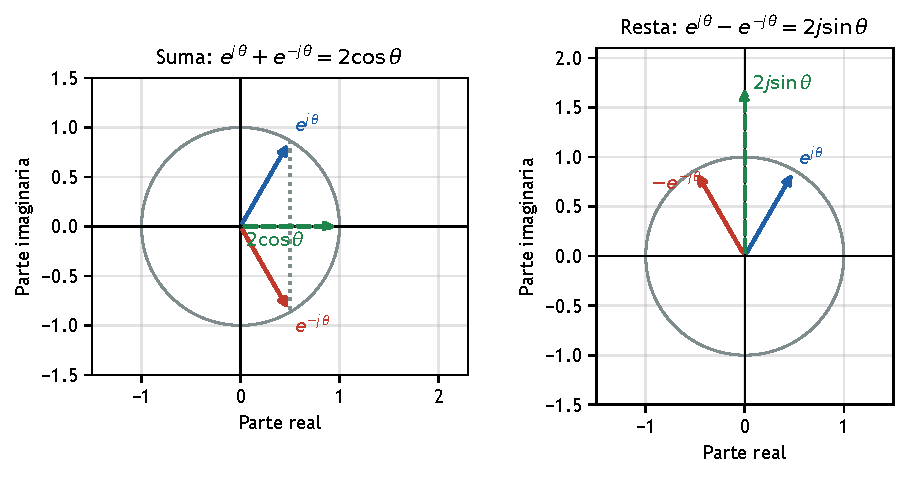
\includegraphics[width=0.95\linewidth]{euler_giro.pdf}
\caption{Izquierda: la suma de $e^{j\theta}$ y su conjugada cae sobre el eje real y vale
$2\cos\theta$. Derecha: la diferencia cae sobre el eje imaginario y vale $2j\sen\theta$
(se dibuja $-e^{-j\theta}$ para sumarla a $e^{j\theta}$). Se muestra $\theta=\pi/3$.}
\label{fig:euler}
\end{figure}

\subsection{De la serie trigonométrica a la compleja}
Se toma un término genérico de la serie trigonométrica y se sustituye $\theta=n\omega_0t$:
\begin{align*}
  a_n\cos(n\omega_0t)+b_n\sen(n\omega_0t)
  &=a_n\,\frac{e^{jn\omega_0t}+e^{-jn\omega_0t}}{2}
   +b_n\,\frac{e^{jn\omega_0t}-e^{-jn\omega_0t}}{2j}
\end{align*}
Se distribuye y se agrupan, por separado, las exponenciales de exponente positivo y negativo:
\begin{equation*}
  =\left(\frac{a_n}{2}+\frac{b_n}{2j}\right)e^{jn\omega_0t}
   +\left(\frac{a_n}{2}-\frac{b_n}{2j}\right)e^{-jn\omega_0t}
\end{equation*}
Con $\dfrac{1}{j}=-j$, es decir $\dfrac{b_n}{2j}=-\dfrac{jb_n}{2}$:
\begin{equation*}
  =\underbrace{\frac{a_n-jb_n}{2}}_{C_n}\,e^{jn\omega_0t}
   +\underbrace{\frac{a_n+jb_n}{2}}_{C_{-n}}\,e^{-jn\omega_0t}
\end{equation*}
El primer paréntesis multiplica a la exponencial de frecuencia $+n\omega_0$ y es, por
definición de la serie compleja, $C_n$; el segundo multiplica a la de $-n\omega_0$ y es
$C_{-n}$:
\begin{equation*}
  \boxed{C_n=\frac{a_n-jb_n}{2}}\qquad\qquad\boxed{C_{-n}=\frac{a_n+jb_n}{2}}
\end{equation*}
y además $\dfrac{a_0}{2}=C_0$.

\textbf{¿Por qué la frecuencia positiva lleva el signo menos y la negativa el signo más?}
Porque el coseno aporta $+\tfrac{1}{2}$ a \emph{ambas} exponenciales (es par), mientras que
el seno aporta $+\tfrac{1}{2j}$ a la positiva y $-\tfrac{1}{2j}$ a la negativa (es impar).
Al escribir $\tfrac{1}{2j}=-\tfrac{j}{2}$, el $+\tfrac{1}{2j}$ de la frecuencia positiva se
vuelve $-\tfrac{j}{2}b_n$, y el $-\tfrac{1}{2j}$ de la negativa se vuelve $+\tfrac{j}{2}b_n$.
El signo viene de la \textbf{imparidad del seno}.

\subsection{La relación inversa}
Se parte de $C_n=\dfrac{a_n-jb_n}{2}$ y $C_{-n}=\dfrac{a_n+jb_n}{2}$.

\textbf{Sumando:}
$\;C_n+C_{-n}=\dfrac{a_n-jb_n+a_n+jb_n}{2}=\dfrac{2a_n}{2}$, es decir
\begin{equation*}
  \boxed{a_n=C_n+C_{-n}}
\end{equation*}
\textbf{Restando:}
$\;C_n-C_{-n}=\dfrac{a_n-jb_n-a_n-jb_n}{2}=\dfrac{-2jb_n}{2}=-jb_n$. Despejando $b_n$ y
usando $\dfrac{1}{-j}=j$:
\begin{equation*}
  \boxed{b_n=j\,(C_n-C_{-n})}
\end{equation*}
Estas fórmulas permiten volver de la representación compleja a la trigonométrica.

\subsection{Aplicación al ejercicio}
Con $a_n=0$ y $b_n=\dfrac{2(-1)^{n+1}}{n}$, en $C_n=\dfrac{a_n-jb_n}{2}$:
\begin{equation*}
  C_n=\frac{0-j\left(\dfrac{2(-1)^{n+1}}{n}\right)}{2}=-\frac{j(-1)^{n+1}}{n}
\end{equation*}
Como $(-1)^{n+1}=-(-1)^{n}$:
\begin{equation*}
  C_n=-\frac{j\cdot\big(-(-1)^{n}\big)}{n}=\boxed{\frac{j(-1)^{n}}{n}}
\end{equation*}
Es \textbf{idéntico} al resultado de la integración exponencial directa
(sección~\ref{sec:c0} y anteriores): los dos métodos producen la misma serie.

\subsection{Verificación de que ambas series son la misma señal}
En la serie compleja se agrupan los términos $n$ y $-n$ ($n\ge 1$). Se sabe que
$C_n=\dfrac{j(-1)^{n}}{n}$ y
$C_{-n}=\dfrac{j(-1)^{-n}}{-n}=-\dfrac{j(-1)^{n}}{n}$, pues $(-1)^{-n}=(-1)^{n}$:
\begin{equation*}
  C_ne^{jnt}+C_{-n}e^{-jnt}=\frac{j(-1)^{n}}{n}\left(e^{jnt}-e^{-jnt}\right)
\end{equation*}
Por la identidad del seno, $e^{jnt}-e^{-jnt}=2j\sen(nt)$:
\begin{equation*}
  =\frac{j(-1)^{n}}{n}\cdot 2j\sen(nt)
  =\frac{2j^{2}(-1)^{n}}{n}\sen(nt)
  =\frac{-2(-1)^{n}}{n}\sen(nt)
  =\frac{2(-1)^{n+1}}{n}\sen(nt)
\end{equation*}
que es exactamente $b_n\sen(nt)$. Sumando sobre todos los $n\ge 1$ se recupera la serie
trigonométrica:
\begin{equation*}
  \sum_{n\neq 0}C_ne^{jnt}=\sum_{n=1}^{\infty}\Big(C_ne^{jnt}+C_{-n}e^{-jnt}\Big)
  =2\sum_{n=1}^{\infty}\frac{(-1)^{n+1}}{n}\sen(nt)\qquad\blacksquare
\end{equation*}
Las dos series representan la misma señal. Numéricamente, con $N=50$ armónicos, la serie
compleja tiene parte imaginaria máxima de \num{2e-16} y difiere de la trigonométrica en
menos de \num{5e-15}.

\FloatBarrier
%=======================================================================
\section{Frecuencias positivas y negativas}\label{sec:frecuencias}
%=======================================================================
En la serie compleja el índice $n$ indica \textbf{qué armónico} es y \textbf{en qué
sentido gira}:

\begin{table}[H]
\centering
\caption{Significado del signo del índice $n$.}
\renewcommand{\arraystretch}{1.5}
\begin{tabular}{llcl}
\toprule
\textbf{Índice} & \textbf{Exponencial} & \textbf{Frecuencia} & \textbf{Significado}\\
\midrule
$n>0$ & $e^{+jn\omega_0t}$ & $+n\omega_0$ & gira en sentido \textbf{antihorario}\\
$n<0$ & $e^{-j|n|\omega_0t}$ & $-|n|\omega_0$ & gira en sentido \textbf{horario}\\
$n=0$ & $e^{0}=1$ & $0$ & no gira: componente \textbf{continua} ($C_0$)\\
\bottomrule
\end{tabular}
\end{table}

\subsection{\texorpdfstring{$e^{j\omega t}$}{e^(jwt)} frente a \texorpdfstring{$e^{-j\omega t}$}{e^(-jwt)}}
Por Euler: $e^{j\omega t}=\cos(\omega t)+j\sen(\omega t)$ y
$e^{-j\omega t}=\cos(\omega t)-j\sen(\omega t)$.

\begin{table}[H]
\centering
\caption{Las dos exponenciales de frecuencia $\pm\omega$.}
\renewcommand{\arraystretch}{1.5}
\begin{tabular}{lcc}
\toprule
 & $e^{j\omega t}$ & $e^{-j\omega t}$\\
\midrule
Parte real & $\cos(\omega t)$ & $\cos(\omega t)$\\
Parte imaginaria & $+\sen(\omega t)$ & $-\sen(\omega t)$\\
Sentido de giro & antihorario & horario\\
\bottomrule
\end{tabular}
\end{table}

Ambas tienen la \textbf{misma parte real} y partes imaginarias \textbf{opuestas}: una es
la \textbf{conjugada} de la otra, $e^{-j\omega t}=\big(e^{j\omega t}\big)^{*}$. Son dos
puntos que giran sobre la misma circunferencia unitaria en sentidos contrarios, siempre
simétricos respecto al eje real (figura~\ref{fig:euler}).

\begin{notatec}{las frecuencias negativas no son físicas}
No existe un oscilador con ``$-3$~Hz''. Las frecuencias negativas son una consecuencia de
la \emph{notación}: para escribir un coseno o un seno reales con exponenciales complejas
hacen falta \textbf{dos}, una girando a cada lado, de modo que sus partes imaginarias se
cancelen y la suma sea real. La frecuencia negativa es el costo de usar la exponencial
compleja, que es mucho más cómoda para operar que senos y cosenos por separado.
\end{notatec}

\subsection{Simetría conjugada para señales reales}
Si $f(t)$ es \textbf{real}, entonces $f(t)=f(t)^{*}$. Se conjuga la serie compleja (el
conjugado de una suma es la suma de los conjugados y
$\big(e^{jn\omega_0t}\big)^{*}=e^{-jn\omega_0t}$):
\begin{equation*}
  f(t)=\sum_{n}C_ne^{jn\omega_0t}\;\Rightarrow\;
  f(t)^{*}=\sum_{n}C_n^{*}\,e^{-jn\omega_0t}=\sum_{m}C_{-m}^{*}\,e^{jm\omega_0t}
\end{equation*}
(en la última igualdad se renombra $m=-n$). Para que $f(t)=f(t)^{*}$ los coeficientes de
$e^{jm\omega_0t}$ deben coincidir: $C_m=C_{-m}^{*}$, es decir
\begin{equation*}
  \boxed{C_{-n}=C_n^{*}}
\end{equation*}
El asterisco indica el \textbf{conjugado complejo} (cambiar $j$ por $-j$). También se ve en
la sección~\ref{sec:equivalencia}: $C_n=\dfrac{a_n-jb_n}{2}$ y $C_{-n}=\dfrac{a_n+jb_n}{2}$
son conjugados porque $a_n$ y $b_n$ son reales.

\begin{table}[H]
\centering
\caption{Simetría conjugada en este ejercicio, con $C_n=\dfrac{j(-1)^{n}}{n}$.}
\renewcommand{\arraystretch}{1.6}
\begin{tabular}{cccc}
\toprule
$n$ & $C_n$ & $C_{-n}$ & ¿$C_{-n}=C_n^{*}$?\\
\midrule
$1$ & $\dfrac{j(-1)}{1}=-j$ & $j$ & sí: $(-j)^{*}=j$\\
$2$ & $\dfrac{j(+1)}{2}=\dfrac{j}{2}$ & $-\dfrac{j}{2}$ & sí: $\left(\dfrac{j}{2}\right)^{*}=-\dfrac{j}{2}$\\
\bottomrule
\end{tabular}
\end{table}

La suma de un número complejo y su conjugado es el doble de su parte real,
$z+z^{*}=2\Real\{z\}$. Por eso cada par de exponenciales produce una onda \textbf{real}:
\begin{equation*}
  C_ne^{jnt}+C_{-n}e^{-jnt}=2\Real\{C_ne^{jnt}\}
\end{equation*}
\begin{ejemplo}{primer armónico}
Con $n=1$ y $C_1=-j$:
$\;2\Real\{-j(\cos t+j\sen t)\}=2\Real\{-j\cos t+\sen t\}=2\sen t$.
Es exactamente el primer armónico de la serie trigonométrica.
\end{ejemplo}

\FloatBarrier
%=======================================================================
\section{Reconstrucción del seno y del coseno}
%=======================================================================

\subsection{El seno}
Para $f(t)=\sen(\omega_0t)$, por la identidad de Euler del seno y con
$\dfrac{1}{2j}=-\dfrac{j}{2}$:
\begin{equation*}
  \sen(\omega_0t)=\frac{e^{j\omega_0t}-e^{-j\omega_0t}}{2j}
  =\frac{1}{2j}e^{j\omega_0t}-\frac{1}{2j}e^{-j\omega_0t}
  =\boxed{-\frac{j}{2}\,e^{j\omega_0t}+\frac{j}{2}\,e^{-j\omega_0t}}
\end{equation*}
Comparando con $f(t)=\sum C_ne^{jn\omega_0t}$:
\begin{equation*}
  C_1=-\frac{j}{2},\qquad C_{-1}=\frac{j}{2},\qquad C_n=0\ \text{para el resto}
\end{equation*}
Un seno \textbf{necesita ambas frecuencias} ($+\omega_0$ y $-\omega_0$): cada exponencial
por separado es compleja, y solo la combinación con coeficientes conjugados ($-\tfrac{j}{2}$
y $+\tfrac{j}{2}$) tiene parte imaginaria nula. Los coeficientes son \textbf{imaginarios
puros} y de \textbf{signo opuesto} (antisimétricos): es la huella de una función
\textbf{impar}. Concuerda con el ejercicio: el primer armónico de $f(t)=t$ es $2\sen t$,
con $C_1=2\cdot\left(-\tfrac{j}{2}\right)=-j$.

\subsection{El coseno}
Para $f(t)=\cos(\omega_0t)$:
\begin{equation*}
  \cos(\omega_0t)=\frac{e^{j\omega_0t}+e^{-j\omega_0t}}{2}
  =\boxed{\frac{1}{2}\,e^{j\omega_0t}+\frac{1}{2}\,e^{-j\omega_0t}}
  \qquad C_1=\frac{1}{2},\quad C_{-1}=\frac{1}{2}
\end{equation*}
Los coeficientes son \textbf{reales} e \textbf{iguales} (simétricos): son conjugados
(porque $\tfrac{1}{2}$ es su propio conjugado) y la suma es real porque las partes
imaginarias se cancelan. Es la huella de una función \textbf{par}.

\begin{notatec}{par frente a impar}
La señal par (coseno) da coeficientes reales y simétricos, $C_{-n}=C_n$; la impar (seno)
da coeficientes imaginarios y antisimétricos, $C_{-n}=-C_n$. Nuestro $f(t)=t$ es impar,
y por eso sus $C_n$ son imaginarios puros con $C_{-n}=-C_n$.
\end{notatec}

\FloatBarrier
%=======================================================================
\section{Tabla comparativa de coeficientes}
%=======================================================================

\subsection{Armónicos positivos}
Cada columna se obtiene así: $a_n=0$ (sección~IV, paridad); $b_n=\dfrac{2(-1)^{n+1}}{n}$;
y $C_n=\dfrac{a_n-jb_n}{2}=-\dfrac{j\,b_n}{2}$, o directamente $C_n=\dfrac{j(-1)^{n}}{n}$.

\begin{table}[H]
\centering
\caption{Coeficientes de los cinco primeros armónicos positivos.}
\renewcommand{\arraystretch}{1.6}
\begin{tabular}{cccc}
\toprule
$n$ & $a_n$ & $b_n$ & $C_n=-\dfrac{j\,b_n}{2}$\\
\midrule
1 & 0 & $2$ & $-j$\\
2 & 0 & $-1$ & $\dfrac{j}{2}$\\
3 & 0 & $\dfrac{2}{3}$ & $-\dfrac{j}{3}$\\
4 & 0 & $-\dfrac{1}{2}$ & $\dfrac{j}{4}$\\
5 & 0 & $\dfrac{2}{5}$ & $-\dfrac{j}{5}$\\
\bottomrule
\end{tabular}
\end{table}

\begin{ejemplo}{comprobación de la fila $n=3$}
$b_3=2(-1)^{4}/3=\tfrac{2}{3}$ y $C_3=-j\cdot\tfrac{2}{3}/2=-\tfrac{j}{3}$. Directamente:
$C_3=j(-1)^{3}/3=-\tfrac{j}{3}$. Coinciden.
\end{ejemplo}

\subsection{Armónicos negativos}
Como $a_n=0$, $C_{-n}=\dfrac{a_n+jb_n}{2}=\dfrac{jb_n}{2}=-C_n$, que equivale a $C_{-n}=C_n^{*}$.

\begin{table}[H]
\centering
\caption{Coeficientes de los cinco primeros armónicos negativos.}
\renewcommand{\arraystretch}{1.6}
\begin{tabular}{cc}
\toprule
$n$ & $C_n$\\
\midrule
$-1$ & $j$\\
$-2$ & $-\dfrac{j}{2}$\\
$-3$ & $\dfrac{j}{3}$\\
$-4$ & $-\dfrac{j}{4}$\\
$-5$ & $\dfrac{j}{5}$\\
\bottomrule
\end{tabular}
\end{table}

\textbf{Simetría conjugada:} cada fila negativa es el conjugado de la positiva con el mismo
$|n|$: $C_{-1}=j=(-j)^{*}=C_1^{*}$, $C_{-2}=-\tfrac{j}{2}=\left(\tfrac{j}{2}\right)^{*}=C_2^{*}$,
etc. Como los $C_n$ son imaginarios puros, conjugar equivale a cambiar de signo. Además la
magnitud $|C_n|=1/|n|$ es la misma a ambos lados: \textbf{el espectro de magnitud es par;
el de fase es impar} (figura~\ref{fig:espectro}).

\begin{figure}[H]
\centering
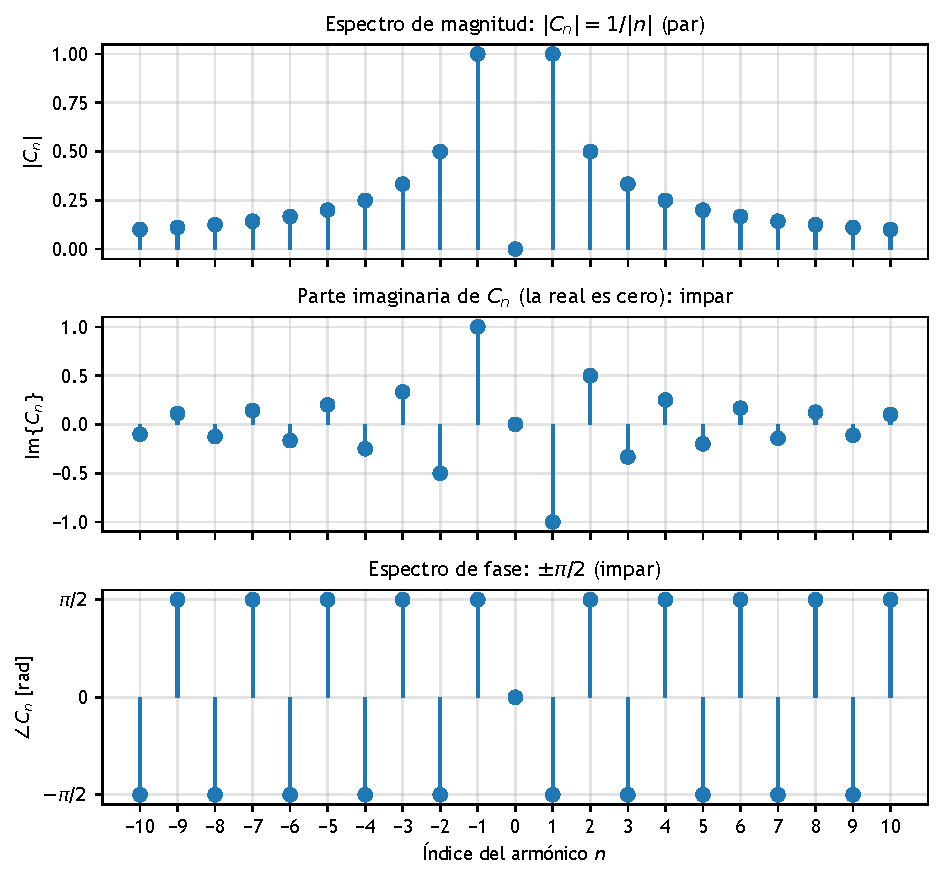
\includegraphics[width=0.9\linewidth]{espectro.pdf}
\caption{Espectro de $f(t)=t$ para $n=-10,\dots,10$. La magnitud $|C_n|=1/|n|$ es par; la
fase vale $\mp\pi/2$ según el signo de $(-1)^{n}/n$ y es impar. En $n=0$ todo es cero
($C_0=0$).}
\label{fig:espectro}
\end{figure}

\FloatBarrier
%=======================================================================
\section{Aproximación con los primeros armónicos}
%=======================================================================
Con cinco armónicos:
\begin{equation*}
  f_5(t)=2\sen t-\sen 2t+\frac{2}{3}\sen 3t-\frac{1}{2}\sen 4t+\frac{2}{5}\sen 5t
\end{equation*}
y, en general, la \textbf{suma parcial} con $N$ armónicos es
\begin{equation*}
  f_N(t)=2\sum_{n=1}^{N}\frac{(-1)^{n+1}}{n}\sen(nt)
\end{equation*}
\textbf{Qué ocurre al aumentar $N$.} Cada armónico añadido mejora el ajuste: la
aproximación se parece cada vez más a la rampa y el error medio disminuye
(figura~\ref{fig:convergencia}). Los armónicos de orden alto tienen amplitud $2/n$ pequeña,
así que solo corrigen detalles finos y los saltos.

\begin{figure}[H]
\centering
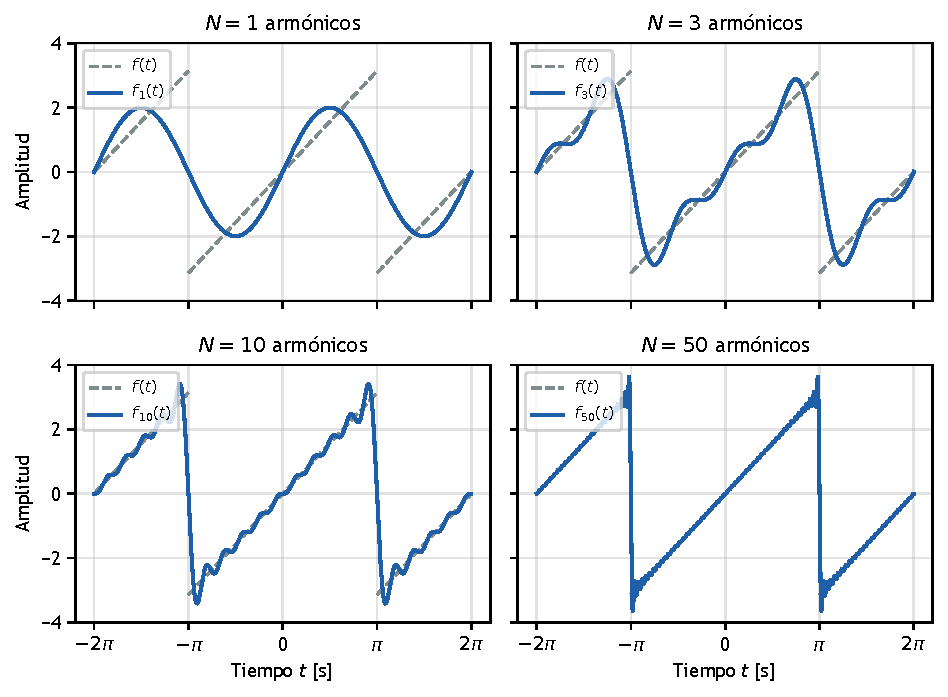
\includegraphics[width=0.95\linewidth]{convergencia.pdf}
\caption{Suma parcial $f_N(t)$ para $N=1,3,10$ y $50$. Con $N=50$ la serie es casi la rampa;
junto a los saltos persiste una oscilación.}
\label{fig:convergencia}
\end{figure}

\textbf{Convergencia.}
\begin{itemize}
    \item En los puntos donde $f$ es \textbf{continua} ($t\neq\pm\pi,\pm3\pi,\dots$),
          $f_N(t)\to f(t)$ cuando $N\to\infty$.
    \item En los \textbf{saltos} (aquí en $t=\pm\pi$, donde la señal pasa de $+\pi$ a $-\pi$)
          la serie converge al \textbf{promedio de los límites laterales}:
\end{itemize}
\begin{equation*}
  f(\pi)=\frac{f(\pi^{-})+f(\pi^{+})}{2}=\frac{\pi+(-\pi)}{2}=0
\end{equation*}
Se comprueba directamente: en $t=\pi$ todos los términos valen $\sen(n\pi)=0$, así que la
serie vale $0$.

\subsection{Fenómeno de Gibbs}
Cerca de un salto las sumas parciales \textbf{sobrepasan} el valor de la señal formando una
oscilación: el pico alcanza alrededor de un \textbf{9~\%} del tamaño del salto (aquí, del
salto de $2\pi$) y \textbf{no desaparece al aumentar $N$}; solo se vuelve más angosto y se
pega al punto de discontinuidad (figura~\ref{fig:gibbs}). Es la consecuencia de intentar
construir un salto abrupto con funciones suaves.

\begin{figure}[H]
\centering
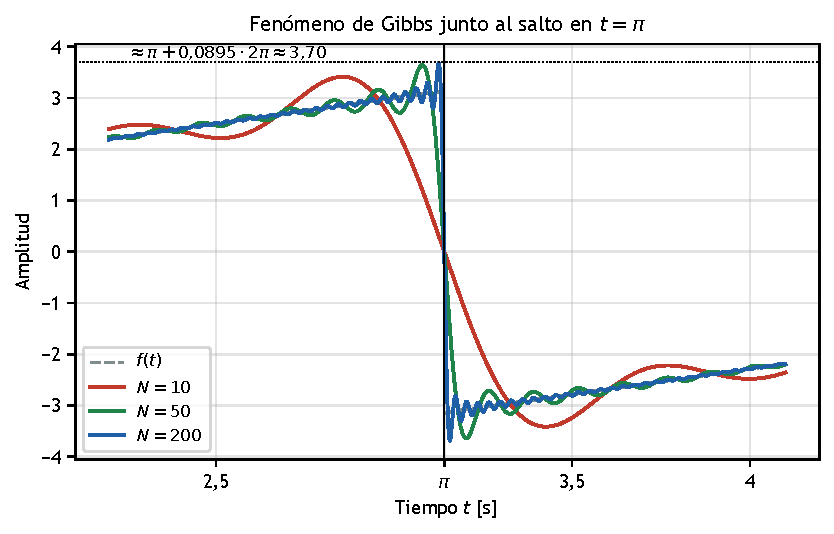
\includegraphics[width=0.9\linewidth]{gibbs.pdf}
\caption{Zona junto al salto en $t=\pi$ para $N=10,50$ y $200$. El pico se estrecha, pero su
altura (alrededor de $3{,}70$) no baja.}
\label{fig:gibbs}
\end{figure}

\FloatBarrier
%=======================================================================
\section{Código Python}
%=======================================================================
El siguiente código genera la señal, calcula la aproximación con $N$ armónicos y
grafica ambas. Se cambia \py{N\_ARMONICOS} para ver el efecto de añadir armónicos. Corre
en Google Colab sin instalar nada (NumPy y Matplotlib ya vienen incluidos).

\begin{Verbatim}
import numpy as np
import matplotlib.pyplot as plt

plt.rcParams["axes.grid"] = True

N_ARMONICOS = 5      # <-- modifica este valor: 1, 3, 5, 10, 50 ...

def senal_original(t):
    """f(t) = t en (-pi, pi), repetida con período 2*pi (diente de sierra)."""
    return np.mod(t + np.pi, 2 * np.pi) - np.pi

def aproximacion(t, N):
    """Suma parcial f_N(t) = 2 * sum_{n=1}^{N} (-1)^(n+1)/n * sin(n t)."""
    n = np.arange(1, N + 1).reshape(-1, 1)     # columna n = 1..N
    bn = 2 * (-1.0) ** (n + 1) / n             # coeficientes b_n
    return np.sum(bn * np.sin(n * t), axis=0)  # suma sobre los armónicos

def graficar(N):
    """Dibuja la señal original y su aproximación con N armónicos."""
    t = np.linspace(-3 * np.pi, 3 * np.pi, 4000)
    plt.plot(t, senal_original(t), label="f(t) original")
    plt.plot(t, aproximacion(t, N), label=f"Serie con N = {N} armónicos")
    plt.title(f"Serie de Fourier de f(t) = t con N = {N} armónicos")
    plt.xlabel("Tiempo t [s]")
    plt.ylabel("Amplitud")
    plt.legend()

plt.figure(figsize=(10, 4.5))
graficar(N_ARMONICOS)
plt.show()
\end{Verbatim}

\begin{notatec}{sin bucles}
La suma sobre los armónicos se hace con \emph{broadcasting} de NumPy: $n$ se declara como
\textbf{columna} (\py{reshape(-1, 1)}) y \py{t} como fila, de modo que
\py{n * t} es una matriz con un renglón por armónico y \py{np.sum(..., axis=0)} los
suma. Es el mismo criterio de los notebooks de la Semana 4: se enseña Python, no se
estorba con bucles. En el notebook \texttt{01\_Serie\_trigonometrica\_y\_compleja.ipynb}
están además las verificaciones numéricas de todos los coeficientes.
\end{notatec}

\FloatBarrier
%=======================================================================
\section{Conclusiones}
%=======================================================================
\begin{itemize}
    \item \textbf{Método trigonométrico.} Como $f(t)=t$ es impar, $a_0=0$ y $a_n=0$ por
          paridad; solo sobreviven los senos, con $b_n=\dfrac{2(-1)^{n+1}}{n}$. El cálculo
          exige integración por partes en el semiperíodo $[0,\pi]$.
    \item \textbf{Método complejo.} Una sola integral,
          $C_n=\dfrac{1}{2\pi}\displaystyle\int_{-\pi}^{\pi}te^{-jnt}\,dt$, entrega
          $C_n=\dfrac{j(-1)^{n}}{n}$ para $n\neq0$, y $C_0=0$ se calcula aparte. El mismo
          procedimiento sirve para cualquier $n$, positivo o negativo.
    \item \textbf{Por qué coinciden.} Las identidades de Euler convierten cada $\cos$ y
          $\sen$ en dos exponenciales; al agrupar queda $C_n=\dfrac{a_n-jb_n}{2}$ y
          $C_{-n}=\dfrac{a_n+jb_n}{2}$. Son dos escrituras de la misma suma.
    \item \textbf{Relación de coeficientes.} $a_n=C_n+C_{-n}$, $b_n=j(C_n-C_{-n})$ y
          $C_0=a_0/2$.
    \item \textbf{Frecuencias positivas y negativas.} Son exponenciales que giran en
          sentidos opuestos; no son frecuencias físicas negativas sino la forma de
          representar un seno o un coseno real como suma de dos exponenciales conjugadas.
    \item \textbf{Simetría conjugada.} Si la señal es real, $C_{-n}=C_n^{*}$: eso garantiza
          que las partes imaginarias se cancelen al sumar cada par.
    \item \textbf{Cuándo usar cada una.} La forma \textbf{trigonométrica} es más intuitiva
          y conviene para ver amplitudes de senos y cosenos o para aprovechar la paridad.
          La \textbf{compleja} es más compacta, trata todos los armónicos con una sola
          fórmula y es la que se generaliza a la transformada de Fourier; es la preferida
          para el análisis de sistemas.
\end{itemize}

\FloatBarrier
%=======================================================================
\section{Fórmulas fundamentales}
%=======================================================================
\begin{table}[H]
\centering
\caption{Resumen de fórmulas.}
\renewcommand{\arraystretch}{1.9}
\begin{tabularx}{\textwidth}{>{\raggedright\arraybackslash}p{3.8cm}X}
\toprule
\textbf{Concepto} & \textbf{Expresión}\\
\midrule
Frecuencia angular fundamental & $\omega_0=\dfrac{2\pi}{T}$\\
Serie trigonométrica & $f(t)=\dfrac{a_0}{2}+\displaystyle\sum_{n=1}^{\infty}\big[a_n\cos(n\omega_0t)+b_n\sen(n\omega_0t)\big]$\\
Coeficientes trigonométricos &
  $a_0=\dfrac{2}{T}\displaystyle\int_{-T/2}^{T/2}\!f\,dt$,\quad
  $a_n=\dfrac{2}{T}\displaystyle\int_{-T/2}^{T/2}\!f\cos(n\omega_0t)\,dt$,\quad
  $b_n=\dfrac{2}{T}\displaystyle\int_{-T/2}^{T/2}\!f\sen(n\omega_0t)\,dt$\\
Serie compleja & $f(t)=\displaystyle\sum_{n=-\infty}^{\infty}C_ne^{jn\omega_0t}$\\
Coeficiente complejo & $C_n=\dfrac{1}{T}\displaystyle\int_{-T/2}^{T/2}f(t)e^{-jn\omega_0t}\,dt$\\
Euler & $e^{j\theta}=\cos\theta+j\sen\theta$\\
Coseno y seno & $\cos\theta=\dfrac{e^{j\theta}+e^{-j\theta}}{2}$,\quad $\sen\theta=\dfrac{e^{j\theta}-e^{-j\theta}}{2j}$\\
De trigonométrica a compleja & $C_n=\dfrac{a_n-jb_n}{2}$,\quad $C_{-n}=\dfrac{a_n+jb_n}{2}$,\quad $C_0=\dfrac{a_0}{2}$\\
De compleja a trigonométrica & $a_n=C_n+C_{-n}$,\quad $b_n=j(C_n-C_{-n})$\\
Señal real & $C_{-n}=C_n^{*}$\\
Par / impar & par: $b_n=0$ (solo cosenos); impar: $a_n=0$ (solo senos)\\
\textbf{Este ejercicio} ($f=t$, $T=2\pi$) &
  $a_n=0$,\quad $b_n=\dfrac{2(-1)^{n+1}}{n}$,\quad $C_n=\dfrac{j(-1)^{n}}{n}$ ($n\neq0$),\quad $C_0=0$\\
\bottomrule
\end{tabularx}
\end{table}

\FloatBarrier
%=======================================================================
\section*{Apéndice. Identidades útiles}
\addcontentsline{toc}{section}{Apéndice. Identidades útiles}
%=======================================================================
Reúne las identidades que se usan, o que conviene tener a mano, al trabajar con series de
Fourier.

\subsection*{A.1. Números complejos y potencias de \texorpdfstring{$j$}{j}}
\begin{table}[H]
\centering
\renewcommand{\arraystretch}{1.5}
\begin{tabularx}{\textwidth}{>{\raggedright\arraybackslash}p{4.4cm}X}
\toprule
\textbf{Identidad} & \textbf{Expresión}\\
\midrule
Unidad imaginaria & $j^{2}=-1$\\
Inverso de $j$ & $\dfrac{1}{j}=-j$\\
Potencias de $j$ & $j^{0}=1,\;j^{1}=j,\;j^{2}=-1,\;j^{3}=-j,\;j^{4}=1$ (se repite cada 4)\\
Conjugado & $(a+jb)^{*}=a-jb$\\
Módulo & $|a+jb|=\sqrt{a^{2}+b^{2}}=\sqrt{zz^{*}}$\\
Parte real e imaginaria & $\Real\{z\}=\dfrac{z+z^{*}}{2}$,\quad $\Imag\{z\}=\dfrac{z-z^{*}}{2j}$\\
Conjugado de un producto & $(z_1z_2)^{*}=z_1^{*}z_2^{*}$\\
Forma polar & $z=|z|\,e^{j\angle z}$\\
\bottomrule
\end{tabularx}
\end{table}

\subsection*{A.2. Euler y exponenciales complejas}
\begin{table}[H]
\centering
\renewcommand{\arraystretch}{1.5}
\begin{tabularx}{\textwidth}{>{\raggedright\arraybackslash}p{4.4cm}X}
\toprule
\textbf{Identidad} & \textbf{Expresión}\\
\midrule
Euler & $e^{j\theta}=\cos\theta+j\sen\theta$\\
Conjugada & $\big(e^{j\theta}\big)^{*}=e^{-j\theta}$\\
Módulo unitario & $|e^{j\theta}|=1$\\
Producto & $e^{j\alpha}e^{j\beta}=e^{j(\alpha+\beta)}$\\
De Moivre & $\big(e^{j\theta}\big)^{n}=e^{jn\theta}=\cos(n\theta)+j\sen(n\theta)$\\
Valores notables & $e^{j0}=1,\;e^{j\pi/2}=j,\;e^{j\pi}=-1,\;e^{j3\pi/2}=-j,\;e^{j2\pi}=1$\\
Periodicidad & $e^{j(\theta+2\pi)}=e^{j\theta}$\\
Para $n$ entero & $e^{jn\pi}=e^{-jn\pi}=(-1)^{n}$,\quad $e^{jn2\pi}=1$\\
\bottomrule
\end{tabularx}
\end{table}

\subsection*{A.3. Trigonometría}
\begin{table}[H]
\centering
\renewcommand{\arraystretch}{1.5}
\begin{tabularx}{\textwidth}{>{\raggedright\arraybackslash}p{4.4cm}X}
\toprule
\textbf{Identidad} & \textbf{Expresión}\\
\midrule
Pitágoras & $\sen^{2}\theta+\cos^{2}\theta=1$\\
Paridad & $\cos(-\theta)=\cos\theta$,\quad $\sen(-\theta)=-\sen\theta$\\
Desfase de $\pi/2$ & $\sen\theta=\cos\!\left(\theta-\tfrac{\pi}{2}\right)$\\
Suma de ángulos (seno) & $\sen(\alpha\pm\beta)=\sen\alpha\cos\beta\pm\cos\alpha\sen\beta$\\
Suma de ángulos (coseno) & $\cos(\alpha\pm\beta)=\cos\alpha\cos\beta\mp\sen\alpha\sen\beta$\\
Ángulo doble & $\sen2\theta=2\sen\theta\cos\theta$,\quad $\cos2\theta=\cos^{2}\theta-\sen^{2}\theta$\\
Cuadrados & $\sen^{2}\theta=\dfrac{1-\cos2\theta}{2}$,\quad $\cos^{2}\theta=\dfrac{1+\cos2\theta}{2}$\\
Producto a suma & $\sen\alpha\sen\beta=\tfrac{1}{2}[\cos(\alpha-\beta)-\cos(\alpha+\beta)]$\\
Producto a suma & $\cos\alpha\cos\beta=\tfrac{1}{2}[\cos(\alpha-\beta)+\cos(\alpha+\beta)]$\\
Producto a suma & $\sen\alpha\cos\beta=\tfrac{1}{2}[\sen(\alpha+\beta)+\sen(\alpha-\beta)]$\\
Forma amplitud-fase & $a\cos\theta+b\sen\theta=A\cos(\theta-\varphi)$, con
  $A=\sqrt{a^{2}+b^{2}}$ y $\varphi=\arctan\dfrac{b}{a}$ (si $a>0$)\\
Múltiplos de $\pi$ & $\sen(n\pi)=0$,\quad $\cos(n\pi)=(-1)^{n}$ ($n$ entero)\\
\bottomrule
\end{tabularx}
\end{table}
La forma amplitud-fase es la tercera representación de la serie de Fourier: cada armónico
se escribe como un solo coseno $A_n\cos(n\omega_0t-\varphi_n)$ con
$A_n=\sqrt{a_n^{2}+b_n^{2}}=2|C_n|$. En este ejercicio $A_n=|b_n|=2/n$.

\subsection*{A.4. Paridad e integrales sobre un intervalo simétrico}
\begin{table}[H]
\centering
\renewcommand{\arraystretch}{1.6}
\begin{tabularx}{\textwidth}{>{\raggedright\arraybackslash}p{4.4cm}X}
\toprule
\textbf{Identidad} & \textbf{Expresión}\\
\midrule
Función par & $g(-t)=g(t)\;\Rightarrow\;\displaystyle\int_{-a}^{a}g\,dt=2\int_{0}^{a}g\,dt$\\
Función impar & $g(-t)=-g(t)\;\Rightarrow\;\displaystyle\int_{-a}^{a}g\,dt=0$\\
Producto & par$\cdot$par = par; impar$\cdot$impar = par; par$\cdot$impar = impar\\
Serie de una función par & $b_n=0$ (solo cosenos y término DC)\\
Serie de una función impar & $a_n=0$ (solo senos)\\
Simetría de media onda & si $f(t+T/2)=-f(t)$, solo hay armónicos impares\\
\bottomrule
\end{tabularx}
\end{table}

\subsection*{A.5. Ortogonalidad de los armónicos}
Estas integrales justifican las fórmulas de $a_n$, $b_n$ y $C_n$. Para $m,n$ enteros
positivos y un período completo:
\begin{align*}
  \frac{2}{T}\int_{-T/2}^{T/2}\cos(m\omega_0t)\cos(n\omega_0t)\,dt&=\delta_{mn}
  &\frac{2}{T}\int_{-T/2}^{T/2}\sen(m\omega_0t)\sen(n\omega_0t)\,dt&=\delta_{mn}\\
  \int_{-T/2}^{T/2}\sen(m\omega_0t)\cos(n\omega_0t)\,dt&=0
  &\frac{1}{T}\int_{-T/2}^{T/2}e^{jm\omega_0t}\,e^{-jn\omega_0t}\,dt&=\delta_{mn}
\end{align*}
donde $\delta_{mn}=1$ si $m=n$ y $0$ si $m\neq n$. \textbf{Idea:} multiplicar la serie por
$e^{-jn\omega_0t}$ e integrar ``filtra'' el único término $n$ y anula todos los demás; por
eso $C_n$ se obtiene con esa integral.

\subsection*{A.6. Integrales usadas en el cálculo}
\begin{table}[H]
\centering
\renewcommand{\arraystretch}{1.7}
\begin{tabularx}{\textwidth}{>{\raggedright\arraybackslash}p{4.4cm}X}
\toprule
\textbf{Identidad} & \textbf{Expresión}\\
\midrule
Por partes & $\displaystyle\int u\,dv=uv-\int v\,du$\\
Seno & $\displaystyle\int\sen(nt)\,dt=-\dfrac{\cos(nt)}{n}$\\
Coseno & $\displaystyle\int\cos(nt)\,dt=\dfrac{\sen(nt)}{n}$\\
Exponencial & $\displaystyle\int e^{at}\,dt=\dfrac{e^{at}}{a}$ (con $a=-jn$ en este ejercicio)\\
$t$ por seno & $\displaystyle\int t\sen(nt)\,dt=-\dfrac{t\cos(nt)}{n}+\dfrac{\sen(nt)}{n^{2}}$\\
$t$ por coseno & $\displaystyle\int t\cos(nt)\,dt=\dfrac{t\sen(nt)}{n}+\dfrac{\cos(nt)}{n^{2}}$\\
$t$ por exponencial & $\displaystyle\int te^{at}\,dt=\dfrac{te^{at}}{a}-\dfrac{e^{at}}{a^{2}}$\\
\bottomrule
\end{tabularx}
\end{table}
La última fila resume la sección~V: con $a=-jn$ se tiene $a^{2}=-n^{2}$ y queda
$-\dfrac{te^{-jnt}}{jn}+\dfrac{e^{-jnt}}{n^{2}}$.

\subsection*{A.7. Parseval: potencia de la señal}
La potencia media de una señal periódica se calcula igual en el tiempo y en los coeficientes:
\begin{equation*}
  \boxed{\frac{1}{T}\int_{-T/2}^{T/2}|f(t)|^{2}\,dt=\sum_{n=-\infty}^{\infty}|C_n|^{2}
  =\frac{a_0^{2}}{4}+\frac{1}{2}\sum_{n=1}^{\infty}\left(a_n^{2}+b_n^{2}\right)}
\end{equation*}
Para este ejercicio, por el lado del tiempo:
\begin{equation*}
  \frac{1}{2\pi}\int_{-\pi}^{\pi}t^{2}\,dt=\frac{1}{2\pi}\cdot\frac{2\pi^{3}}{3}=\frac{\pi^{2}}{3}
\end{equation*}
y por el lado de los coeficientes, con $|C_n|=1/|n|$ y $\sum_{n=1}^{\infty}1/n^{2}=\pi^{2}/6$:
\begin{equation*}
  \sum_{n\neq0}\frac{1}{n^{2}}=2\sum_{n=1}^{\infty}\frac{1}{n^{2}}=2\cdot\frac{\pi^{2}}{6}=\frac{\pi^{2}}{3}\;\checkmark
\end{equation*}
Coinciden, lo que confirma los coeficientes por un camino independiente. Además, la potencia
captada por los primeros $N$ armónicos es $2\sum_{n=1}^{N}1/n^{2}$:

\begin{table}[H]
\centering
\caption{Porcentaje de la potencia total $\pi^{2}/3$ que captan los primeros $N$ armónicos.}
\renewcommand{\arraystretch}{1.3}
\begin{tabular}{ccccccc}
\toprule
$N$ & 1 & 3 & 5 & 10 & 50\\
\midrule
Potencia captada & \qty{60.79}{\percent} & \qty{82.75}{\percent} & \qty{88.98}{\percent}
  & \qty{94.21}{\percent} & \qty{98.80}{\percent}\\
\bottomrule
\end{tabular}
\end{table}

\FloatBarrier
%=======================================================================
\section*{Ejercicios propuestos}
\addcontentsline{toc}{section}{Ejercicios propuestos}
%=======================================================================

\subsection*{Parte A. Ejercicios cortos}
Cada uno se resuelve en pocas líneas y practica una sola idea del documento. Las
respuestas de control están al final.

\begin{enumerate}
    \item \textbf{Frecuencias.} Calcula la frecuencia fundamental $f_0$ y la frecuencia
          angular $\omega_0$ de una señal con período $T=4$~s y de otra con
          $T=0{,}02$~s.
          \lineasresp{1}
    \item \textbf{Paridad.} Sin integrar, indica qué coeficientes valen cero en la serie de
          Fourier de cada señal (todas con $T=2\pi$ y definidas en $(-\pi,\pi)$):
          (a)~$f(t)=t^{2}$; (b)~$f(t)=t^{3}$; (c)~$f(t)=5$.
          \lineasresp{2}
    \item \textbf{De trigonométrica a compleja.} Escribe $f(t)=3\cos(2t)+4\sen(2t)$ como
          suma de exponenciales complejas. ¿Cuánto valen $C_2$ y $C_{-2}$?
          \textit{Pista:} usa $C_n=\dfrac{a_n-jb_n}{2}$.
          \lineasresp{2}
    \item \textbf{De compleja a trigonométrica.} Una señal real tiene $C_3=1+2j$. ¿Cuánto
          valen $C_{-3}$, $a_3$ y $b_3$?
          \textit{Pista:} usa $C_{-n}=C_n^{*}$, $a_n=C_n+C_{-n}$ y $b_n=j(C_n-C_{-n})$.
          \lineasresp{2}
    \item \textbf{Convergencia en un salto.} Una señal periódica salta de $2$ a $6$ en
          $t=1$. ¿A qué valor converge su serie de Fourier en $t=1$?
          \lineasresp{1}
\end{enumerate}

\FloatBarrier
\subsection*{Parte B. Ejercicio completo: el mismo recorrido con otra señal}
Repite, con la \textbf{onda cuadrada}, todo el camino que se hizo con la diente de
sierra (figura~\ref{fig:cuadrada}):
\begin{equation*}
  f(t)=\begin{cases}-1, & -\pi<t<0\\[2pt] \;\;\,1, & 0<t<\pi\end{cases}
  \qquad T=2\pi
\end{equation*}

\begin{figure}[!htbp]
\centering
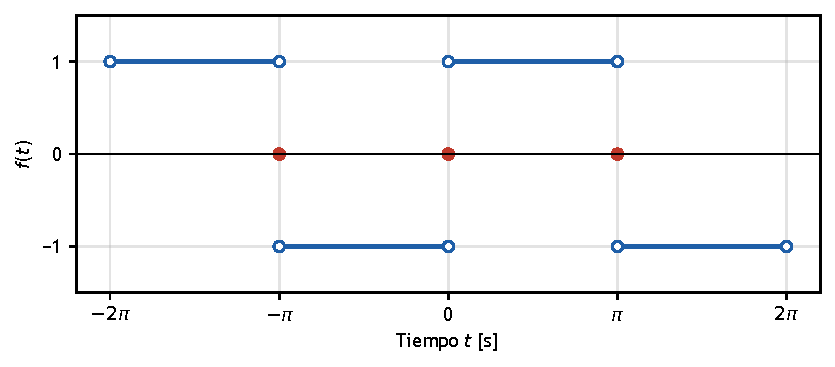
\includegraphics[width=0.85\linewidth]{onda_cuadrada.pdf}
\caption{Onda cuadrada del ejercicio de la Parte~B, con $T=2\pi$.}
\label{fig:cuadrada}
\end{figure}

Esta señal es más sencilla de integrar: \textbf{no necesita integración por partes}, solo la
integral de $\sen(nt)$ y la de $e^{-jnt}$. Se resuelve en este orden:

\begin{enumerate}[label=\textbf{Paso \arabic*.},leftmargin=*,labelsep=0.6em]
    \item \textbf{Preparación.} Calcula $\omega_0$. Decide, \emph{antes de integrar}, si la
          señal es par o impar y qué coeficientes serán cero.
          \lineasresp{2}
    \item \textbf{$a_0$ y $a_n$.} Calcúlalos o justifica con la paridad que son cero.
          \lineasresp{2}
    \item \textbf{$b_n$.} Reduce la integral al tramo $[0,\pi]$, intégrala y evalúa con
          $\cos(n\pi)=(-1)^{n}$. Obtén una expresión \textbf{distinta para $n$ par y para
          $n$ impar}.
          \lineasresp{4}
    \item \textbf{Serie trigonométrica.} Escríbela y desarrolla los tres primeros términos no
          nulos.
          \lineasresp{2}
    \item \textbf{$C_n$ por integración directa.} Parte la integral en dos tramos
          ($-\pi$ a $0$ y $0$ a $\pi$). Calcula $C_0$ aparte.
          \lineasresp{4}
    \item \textbf{Equivalencia.} Comprueba que $C_n=\dfrac{a_n-jb_n}{2}$ da el mismo
          resultado y escribe también $C_{-n}$.
          \lineasresp{2}
    \item \textbf{Tabla.} Completa los coeficientes para $n=1,\dots,5$ y comprueba
          $C_{-n}=C_n^{*}$. La primera fila ya está resuelta como modelo.
\end{enumerate}

\begin{table}[H]
\centering
\caption{Coeficientes de la onda cuadrada (completar).}
\renewcommand{\arraystretch}{2.0}
\begin{tabular}{|c|c|c|c|c|}
\hline
$n$ & $a_n$ & $b_n$ & $C_n$ & $C_{-n}$\\
\hline
1 & $0$ & $\dfrac{4}{\pi}$ & $-\dfrac{2j}{\pi}$ & $\dfrac{2j}{\pi}$\\
\hline
2 & \hspace{1.6cm} & \hspace{1.6cm} & \hspace{1.6cm} & \hspace{1.6cm}\\
\hline
3 & & & &\\
\hline
4 & & & &\\
\hline
5 & & & &\\
\hline
\end{tabular}
\end{table}

\begin{enumerate}[label=\textbf{Paso \arabic*.},leftmargin=*,labelsep=0.6em,start=8]
    \item \textbf{Aproximación.} Completa la plantilla de código de abajo, grafica $f_N$ con
          $N=1,3,10$ y $50$, y responde: ¿cuánto vale la serie en $t=0$? ¿Y en
          $t=\pi/2$? ¿Aparece el fenómeno de Gibbs?
          \lineasresp{3}
\end{enumerate}

\needspace{24\baselineskip}
\begin{Verbatim}
import numpy as np
import matplotlib.pyplot as plt

def onda_cuadrada(t):
    """f(t) = +1 en (0, pi) y -1 en (-pi, 0), repetida con período 2*pi."""
    return np.sign(np.sin(t))

def aproximacion_cuadrada(t, N):
    """Suma parcial con N armónicos."""
    n = np.arange(1, N + 1).reshape(-1, 1)     # columna n = 1..N
    bn = 0 * n          # <-- COMPLETA con tu resultado del paso 3.
                        #     Pista: np.where(n % 2 == 1, valor_impar, valor_par)
    return np.sum(bn * np.sin(n * t), axis=0)

t = np.linspace(-2 * np.pi, 2 * np.pi, 4000)
plt.plot(t, onda_cuadrada(t), label="f(t) original")
plt.plot(t, aproximacion_cuadrada(t, 10), label="Serie con N = 10 armónicos")
plt.title("Onda cuadrada con N = 10 armónicos")
plt.xlabel("Tiempo t [s]"); plt.ylabel("Amplitud"); plt.legend(); plt.show()

print("Serie en t = 0    :", aproximacion_cuadrada(np.array([0.0]), 200)[0])
print("Serie en t = pi/2 :", aproximacion_cuadrada(np.array([np.pi / 2]), 200)[0])
\end{Verbatim}

\begin{notatec}{verificar el resultado}
El notebook \texttt{01\_Serie\_trigonometrica\_y\_compleja.ipynb} trae al final un
\emph{verificador} que calcula numéricamente $a_n$, $b_n$, $C_n$ y $C_{-n}$ de la onda
cuadrada, para comparar con lo obtenido a mano.
\end{notatec}

\newpage
%=======================================================================
\section*{Respuestas de control}
\addcontentsline{toc}{section}{Respuestas de control}
%=======================================================================
Intenta los ejercicios antes de mirar esta página.
\small\setlength{\abovedisplayskip}{3pt}\setlength{\belowdisplayskip}{3pt}

\subsection*{Parte A}
\begin{enumerate}
    \item $T=4$~s: $f_0=\qty{0.25}{\hertz}$ y $\omega_0=\pi/2\approx\qty{1.571}{\radian\per\second}$.
          $\;T=\qty{0.02}{\second}$: $f_0=\qty{50}{\hertz}$ y
          $\omega_0=100\pi\approx\qty{314.16}{\radian\per\second}$.
    \item (a)~$t^{2}$ es par: $b_n=0$ (solo cosenos y término continuo).
          (b)~$t^{3}$ es impar: $a_0=0$ y $a_n=0$ (solo senos).
          (c)~La constante $5$ es par: solo $a_0=10$; todos los $a_n$ y $b_n$ ($n\ge1$) son cero.
    \item $a_2=3$ y $b_2=4$; luego $C_2=\dfrac{3-4j}{2}=1{,}5-2j$ y
          $C_{-2}=\dfrac{3+4j}{2}=1{,}5+2j$.
    \item $C_{-3}=1-2j$; $a_3=C_3+C_{-3}=2$; $b_3=j(C_3-C_{-3})=j\cdot4j=-4$.
    \item Converge al promedio de los límites laterales: $\dfrac{2+6}{2}=4$.
\end{enumerate}

\subsection*{Parte B}
\begin{enumerate}[label=\textbf{Paso \arabic*.},leftmargin=*,labelsep=0.6em]
    \item $\omega_0=\qty{1}{\radian\per\second}$. La señal es \textbf{impar}: $a_0=0$ y $a_n=0$.
    \item $a_0=0$ y $a_n=0$ por paridad.
    \item
          \begin{equation*}
            b_n=\frac{2}{\pi}\int_{0}^{\pi}\sen(nt)\,dt
            =\frac{2}{\pi}\left[-\frac{\cos(nt)}{n}\right]_{0}^{\pi}
            =\frac{2\big(1-(-1)^{n}\big)}{n\pi}
          \end{equation*}
          Para $n$ impar, $b_n=\dfrac{4}{n\pi}$; para $n$ par, $b_n=0$.
    \item $\displaystyle f(t)=\frac{4}{\pi}\left[\sen t+\frac{1}{3}\sen3t+\frac{1}{5}\sen5t+\cdots\right]$.
          Solo hay armónicos \textbf{impares}.
    \item
          \begin{equation*}
            C_n=\frac{1}{2\pi}\left[-\int_{-\pi}^{0}e^{-jnt}dt+\int_{0}^{\pi}e^{-jnt}dt\right]
            =\frac{1-(-1)^{n}}{j\,n\pi}=-\frac{j\big(1-(-1)^{n}\big)}{n\pi}
          \end{equation*}
          Para $n$ impar, $C_n=-\dfrac{2j}{n\pi}$; para $n$ par, $C_n=0$. Además $C_0=0$.
    \item $C_n=\dfrac{0-jb_n}{2}=-\dfrac{j}{2}\cdot\dfrac{4}{n\pi}=-\dfrac{2j}{n\pi}$ ($n$ impar):
          coincide. $C_{-n}=\dfrac{2j}{n\pi}$.
    \item
          \begin{center}
          \small\renewcommand{\arraystretch}{1.35}
          \begin{tabular}{ccccc}
          \toprule
          $n$ & $a_n$ & $b_n$ & $C_n$ & $C_{-n}$\\
          \midrule
          1 & 0 & $\dfrac{4}{\pi}\approx1{,}273$ & $-\dfrac{2j}{\pi}$ & $\dfrac{2j}{\pi}$\\
          2 & 0 & 0 & 0 & 0\\
          3 & 0 & $\dfrac{4}{3\pi}\approx0{,}424$ & $-\dfrac{2j}{3\pi}$ & $\dfrac{2j}{3\pi}$\\
          4 & 0 & 0 & 0 & 0\\
          5 & 0 & $\dfrac{4}{5\pi}\approx0{,}255$ & $-\dfrac{2j}{5\pi}$ & $\dfrac{2j}{5\pi}$\\
          \bottomrule
          \end{tabular}
          \end{center}
    \item En la plantilla: \py{bn = np.where(n \% 2 == 1, 4 / (n * np.pi), 0)}. En $t=0$ la
          serie vale $0$ (promedio de $-1$ y $1$). En $t=\pi/2$ vale $1$:
          $\dfrac{4}{\pi}\left(1-\dfrac{1}{3}+\dfrac{1}{5}-\cdots\right)=\dfrac{4}{\pi}\cdot\dfrac{\pi}{4}=1$.
          Sí aparece Gibbs: junto a cada salto el pico supera a $1$ en cerca del
          9~\% del tamaño del salto ($2$), es decir llega a $\approx1{,}18$, y no baja al
          aumentar $N$.
\end{enumerate}

\end{document}
